\documentclass[11pt,a4paper]{article}
\usepackage[utf8]{inputenc}
\usepackage[T1]{fontenc}
\usepackage{textcomp}
\usepackage[english]{babel}
\usepackage[margin=1.5cm]{geometry}
\usepackage{booktabs}
\usepackage{longtable}
\usepackage{graphicx}
\usepackage{array}
\usepackage{enumitem}
\usepackage{hyperref}
\documentclass[12pt,a4paper]{article}
\usepackage[utf8]{inputenc}
\usepackage[T1]{fontenc}
\usepackage[french]{babel}
\usepackage{lmodern,microtype}
\usepackage[margin=2.5cm]{geometry}
\usepackage{graphicx}
\graphicspath{{images/}}
\usepackage{booktabs}
\usepackage{tabularx}
\usepackage{array}
\usepackage[table]{xcolor}
\usepackage{enumitem}
\usepackage{amsmath}
\usepackage{calc}      
\usepackage{float}
\usepackage{siunitx}
\sisetup{locale=FR}
\usepackage{needspace}
\usepackage{pdfpages}
\usepackage{tikz}
\usetikzlibrary{arrows.meta,positioning}
\usepackage{csquotes}
\usepackage{longtable}
\usepackage{array}
\usepackage{siunitx} 
\usepackage[backend=biber,style=numeric,sorting=none]{biblatex}
\addbibresource{refs.bib}
\usepackage[hidelinks]{hyperref} % Load last


\setlength{\tabcolsep}{4pt}
\renewcommand{\arraystretch}{1.3}
\setlength{\parindent}{0pt}
\setlist{itemsep=2pt,topsep=3pt}

% Placeholder for information still to be filled in
\newcommand{\todo}[1]{\textbf{[TO DO: #1]}}

\newcommand{\risqueentete}{%
  \toprule
  \textbf{Risk} & \textbf{Cause} & \textbf{Consequence} & \textbf{Level} & \textbf{Prevention} \\
  \midrule
  \endfirsthead
  \toprule
  \textbf{Risk} & \textbf{Cause} & \textbf{Consequence} & \textbf{Level} & \textbf{Prevention} \\
  \midrule
  \endhead
  \bottomrule
  \endfoot
}

\begin{document}

\begin{center}
{\Large \textbf{ARGUS Project}}\\[0.3em]
{\large Mission Definition, Payload Description}\\[0.5em]
ARGUS project -- November 2026
\end{center}

\small
\tableofcontents
\normalsize

% ==================================================================
\section{Mission Definition}

\subsection{Studied object / functional mission target}
\textbf{Definitive choice:} space debris in low Earth orbit, a small object (about  less than 1\,kg, aluminium surface) to be tracked and deflected by a CubeSat.

\subsection{Scientific / technological question or aim}
\textbf{Definitive choice:} demonstrate that a 6U CubeSat can detect and track a small debris at short range with a LiDAR, and change its trajectory by laser ablation (target : small $\Delta V$).


\subsection{Main payload}
The main payload of the Argus mission is the debris, which we aim to eject.
The shape of the debris has not been finalized, but it will be a small object weighing less than 1\,kg with an aluminium surface.
The second main payload is the laser, a Class 4 laser with a wavelength of 1064\,nm.

\subsection{Secondary payloads (if any)}
The laser will be guided by a LiDAR (secondary payload) operating at a wavelength of 1550\,nm, equipped with a SPAD detector and a MEMS micro-mirror.
The second secondary payload is a camera with a machine learning algorithm to detect the debris and estimate its orientation.
Thanks to these two instruments, we can track the debris and fire the laser at it.

\subsection{Experts contacted}
Ratio of contacted experts: \todo{X}\,\% (\todo{X} experts contacted out of \todo{Y} experts initially identified).

\todo{table of experts (name, field, topic, contacted or not) -- to be defined once the other subsystem is discussed}
Vincent robert for space mecanique
if u have someone for laser ablation and ml and camera, please contact him
% ==================================================================
\section{Payload Description}
% ---------- Payload ----------

Sizing a LASER-ablation deorbiting system involves a direct physical trade-off:
 the LASER must not destroy the debris through excessive heat input, 
 but must vaporise a very thin layer of its surface to create a propulsive plasma that slows the moving debris. 
 Thus, modifying the orbit of an object (debris) relies on converting the optical energy deposited by laser pulses into the mechanical energy of the plasma jet.

\subsection{LASER Ablation Propulsion}
When a high-intensity LASER beam strikes the surface of a material, 
the optical energy is absorbed instantaneously. 
The temperature of the surface layer rises so rapidly that it undergoes sudden sublimation and becomes a highly energetic plasma. 
This jet of matter is expelled at very high speeds. Under the physical law of conservation of matter, the ejection of matter generates a mechanical recoil force on the target object \cite{Vincent2011}.

\begin{figure}[H]
  \centering
  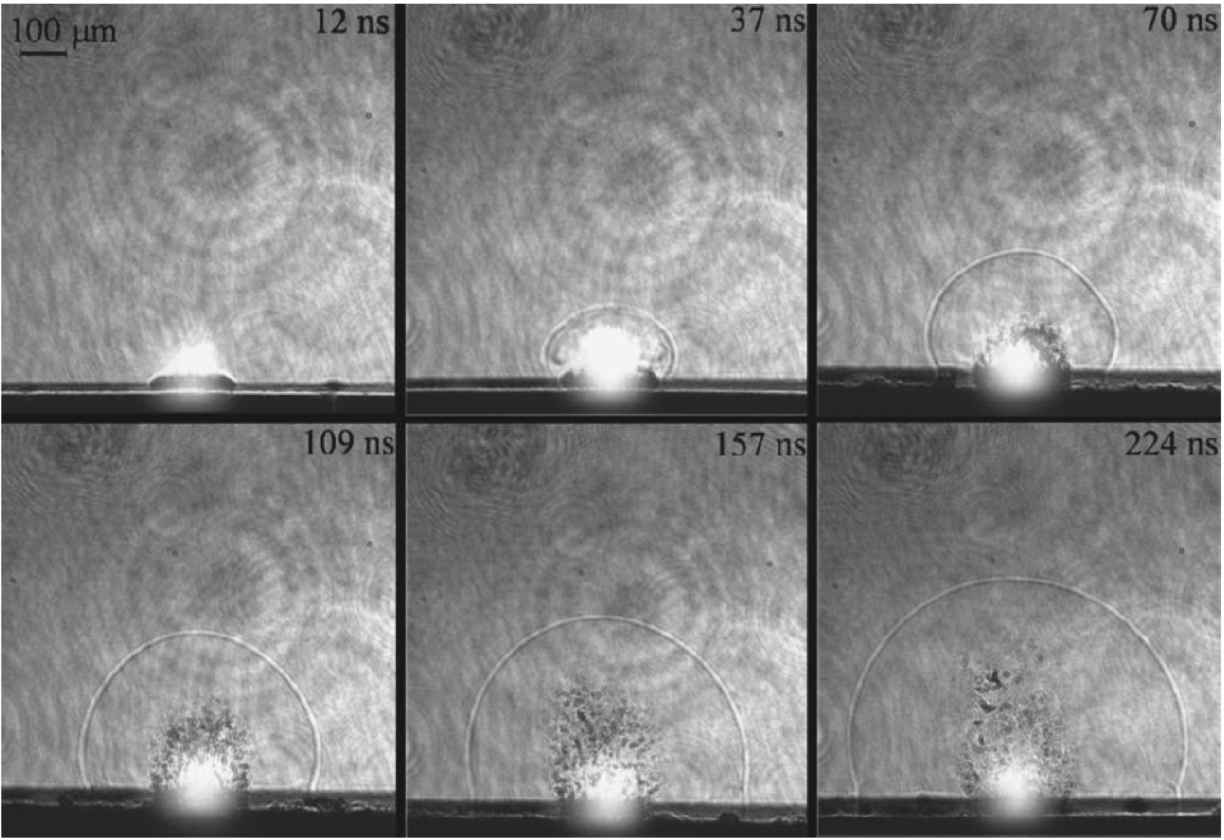
\includegraphics[width=0.8\textwidth,height=7cm,keepaspectratio]{ablation_laser.png}
  \caption{Images of the ablation propulsion process at different times during the laser--aluminium interaction for $\lambda = 1064 nm$ and $\tau = 5ns$. The propagation of the shock wave over time can be observed. \cite{Vincent2011}}
  \label{fig:ablation}
\end{figure}

\subsection{High-Power LASER Characteristics}
In this section, we describe the characteristics of our onboard high-power LASER. 
Selecting the high-power LASER is crucial: if its power or energy is unsuitable, 
it will probably not be possible to initiate the micropropulsion process at the surface of our target (debris).

\begin{enumerate}
    \item \textbf{Choice of LASER type:}\\
    We choose a pulsed LASER rather than a continuous-wave laser. 
    The factors determining this choice are summarised in the table below

    \begin{table}[H]
      \centering
      \caption{Comparison between continuous-wave and pulsed lasers.}
      \begin{tabular}{p{3.5cm} p{5.5cm} p{5.5cm}}
        \toprule
        \textbf{Characteristic} & \textbf{Continuous-wave laser } & \textbf{Pulsed laser} \\
        \midrule
        Effect on debris & Thermal melting  & Plasma ablation (mechanical rocket effect) \\
        Peak power & Equal to average power  & Several megawatts during the pulse \\
        Generated thrust & Almost zero at this power level & Optimal and directional \\
        Risks & High risk of breaking up the debris & Safe, targeted surface action \\
        \bottomrule
      \end{tabular}
    \end{table}

    \item \textbf{Required LASER parameters:}\\
    The wavelength of our high-power LASER is set to $\lambda = $\SI{1064}{\nano\metre} in the infrared, with a pulse duration of \textbf{nanoseconds (ns)}. This choice is primarily based on the absorption characteristics of the material making up our debris, namely aluminium (Al).

    For this CubeSat project using a $6U$ platform firing a LASER at short range, the optimal average power required for our small aluminium debris object, measuring \SIrange{1}{10}{\centi\metre} and weighing $1kg$ is approximately $1000W$. The choice of this operating power is deliberate and results from a specific trade-off validated by orbital mechanics and the physics of laser--matter interaction. The section on project feasibility discusses in detail the importance of reaching this optimal LASER ablation power.

    \begin{table}[H]
      \centering
      \small
      \caption{Ablation laser parameters.}
      \label{tab:laser_ablation}
      \begin{tabular}{p{6cm} p{6cm}}
        \toprule
        \textbf{Parameter} & \textbf{Value} \\
        \midrule
        Wavelength ($\lambda$) & \SI{1064}{\nano\metre} (infrared) \\
        Operating mode & Pulsed \\
        Pulse duration ($\tau$) & Nanosecond (ns) \\
        Average power ($P_{\text{moy}}$) & \SI{1000}{\watt} (\SI{1}{\kilo\watt}) \\
        Repetition rate ($f$) & \SI{3000}{\hertz} (\SI{2}{\kilo\hertz}) \\
        Pulse energy ($E_p$) & \SI{0.5}{\joule} \\
        Peak power ($P_{\text{crête}}$) & \SI{100}{\mega\watt} \\
        Ablation threshold fluence & \SIrange{1}{2}{\joule\per\centi\metre\squared} \\
        Optimal coupling fluence & \SI{5}{\joule\per\centi\metre\squared} \\
        \bottomrule
      \end{tabular}
    \end{table}
\end{enumerate}

\newpage
\subsection{LiDAR for Detection}
To meet the imposed dimensional constraints, we favour a micro-LiDAR over a conventional LiDAR, which would entail higher mass and energy demands. The micro-LiDAR provides optical metrology of the debris: detection, relative position and relative velocity \cite{OpromollaNocerino}. It consists of three main elements:
\begin{itemize}
    \item The emission source, which in our case could be a VCSEL (Vertical Cavity Surface Emitting LASER). These are arrays of miniature semiconductor LASERs. The table below summarises the parameters we consider optimal for defining the LASER source of our micro-LiDAR.

    \begin{table}[H]
      \centering
      \small
      \caption{Micro-LiDAR laser parameters \cite{VCSEL1550_2023}.}
      \label{tab:lidar_laser}
      \begin{tabular}{p{3.3cm} p{4.7cm} p{6.5cm}}
        \toprule
        \textbf{Parameter} & \textbf{Specified value} & \textbf{Purpose in space} \\
        \midrule
        Wavelength & \SI{1550}{\nano\metre} & Prevents blinding by the ablation laser (\SI{1064}{\nano\metre}) \\
        Source type & Pulsed laser diode (InGaAs) & Robustness, extreme compactness \\
        Pulse duration & \SI{3}{\nano\second} & Millimetre-level ranging accuracy \\
        Frequency & \SI{20}{\kilo\hertz} & Smooth real-time target tracking \\
        Pulse energy & \SI{10}{\micro\joule} & Completely harmless to the debris \\
        Electrical power consumption & $\approx\SI{12}{\watt}$ & Fully suited to the constraints of a 6U CubeSat \\
        \bottomrule
      \end{tabular}
    \end{table}

    \item An ultrasensitive SPAD (Single Photon Avalanche Diode) detector. These detectors can detect a single returning photon. The table below summarises the parameters we consider optimal for selecting a suitable detector for our micro-LiDAR \cite{Pellegrini2006}.

    \begin{table}[H]
      \centering
      \small
      \caption{Micro-LiDAR SPAD detector parameters \cite{SPADReview2024}.}
      \label{tab:lidar_spad}
      \begin{tabular}{p{3.3cm} p{4.7cm} p{6.5cm}}
        \toprule
        \textbf{Parameter} & \textbf{Specified value} & \textbf{Purpose in space} \\
        \midrule
        Detector type & SPAD InGaAs/InP & Sensitive at \SI{1550}{\nano\metre}, single-photon detection \\ % to be verified
        Detection efficiency & $\approx\SI{20}{\percent}$ at \SI{1550}{\nano\metre} & Detect the weak signal backscattered by the debris \\ % to be verified
        Timing jitter (\textit{jitter}) & $\approx\SI{200}{\pico\second}$ & Range resolution of a few centimetres \\ % to be verified
        Dark count rate & $\approx\SI{10}{\kilo\hertz}$ (cooled detector) & Limit noise to maintain a good signal-to-noise ratio \\ % to be verified
        Operating mode & Gated (\textit{gated}), synchronised with the pulse & Reduce noise and power consumption \\ % to be verified
        \bottomrule
      \end{tabular}
    \end{table}

    \item MEMS (Micro-Electro-Mecanical System) micromirrors. These oscillating micromirrors are etched into silicon to steer the beam without heavy mechanical components. The table below summarises the parameters we consider optimal for selecting the mirror assembly for our micro-LiDAR \cite{Shea2006}.

    \begin{table}[H]
      \centering
      \small
      \caption{Micro-LiDAR oscillating MEMS micromirror parameters \cite{Liu2022}.}
      \label{tab:lidar_mems}
      \begin{tabular}{p{3.3cm} p{4.7cm} p{6.5cm}}
        \toprule
        \textbf{Parameter} & \textbf{Specified value} & \textbf{Purpose in space} \\
        \midrule
        Scanning mechanism & Resonant MEMS micromirror & Scene scanning without bulky mechanical components \\ % to be verified
        Mirror diameter & $\approx\SI{1}{\milli\metre}$ & Trade-off between optical aperture and resonant frequency \\ % to be verified
        Optical scan angle & $\pm\SI{10}{\degree}$ & Cover the field of view required for target acquisition \\ % to be verified
        Resonant frequency & $\approx\SI{1}{\kilo\hertz}$ & Scan rate compatible with real-time tracking \\ % to be verified
        Electrical power consumption & Less than $\SI{1}{\watt}$ & Compatible with the power budget of a 6U CubeSat \\ % to be verified
        \bottomrule
      \end{tabular}
    \end{table}
\end{itemize}



%\subsection{Functional description of the payloads' behavior}
%%%\todo{complete and check the sequence below}
%\begin{enumerate}
%\item \textbf{Detection:} the LiDAR scans its field of view ($\pm 10^\circ$) and detects the debris.
%\item \textbf{Tracking:} the LiDAR measures the position of the debris and keeps tracking it; the fine pointing mirror is guided by the LiDAR data.
%\item \textbf{Lock check:} firing is authorized only if the target is locked (shutter opened).
%\item \textbf{Firing:} short laser bursts on battery power, ablating the aluminium surface to produce thrust.
%\item \textbf{Monitoring:} the debris is tracked during and after each burst; firing stops automatically in case of anomaly (fluence, loss of tracking).
%\item \textbf{Safe state:} firing inhibited by default outside the contact windows or without lock.
%\end{enumerate}

%\subsection{Quantified description of the payloads' performance}

%\todo{quantified performance table of all payloads -- to be discussed with the other subsystem}



% ==================================================================
\section{System Architecture and Diagrams}

\subsection{Data Management Plan -- functional diagram V1}

\begin{figure}[htbp]
    \centering
    \includegraphics[width=0.8\textwidth]{data_management.png}
    \caption{Data Management Plan -- functional diagram V1.}
    \label{fig:data_management}
\end{figure}

\noindent\textbf{Legend.} The diagram is divided into three phases:
\textit{search of the debris} (detection and localisation),
\textit{calculation after ablation} (check of the laser effect and transmission),
and \textit{analysis of the data on ground}.
Each box is a step of the chain, and the small text next to it gives the equipment
performing the step (onboard computer, lidar, camera, communication board, antenna,
ground station, ground computer, or researcher).
The labels on the arrows give the type of data exchanged:
\textit{picture} (raw camera image),
\textit{position octet} (debris position encoded in bytes),
\textit{octet} (binary data such as measurements and deviation),
\textit{frequency} (radio signal between the antenna and the ground station),
and \textit{text} (final publication).

\subsection{Satellite platform -- functional diagram V1}
\todo{insert the figure (see the ``Examples'' tab)look on miro}

\subsection{Satellite system model V1 (IDM-CIC)}
\todo{insert the screenshot or the link to the IDM-CIC model}

% ==================================================================
\section{Mission Analysis V1}

\todo{orbit and mission phases -- to be discussed with the other subsystem}
\todo{maybe add some seach on procurreezy and vector ifyou have sometjing interresing}

% ==================================================================
\section{Mission Report Summary V1}
\todo{write the summary following the ``Leads for Report Summary'' tab: context, objectives, payloads, architecture, orbit and phases, main risks, schedule}

% ==================================================================
\section{Risk Analysis}

\subsection{Risks related to the power LASER}

\begin{longtable}{>{\raggedright\arraybackslash}p{3.7cm} >{\raggedright\arraybackslash}p{4.2cm} >{\raggedright\arraybackslash}p{3.7cm} >{\centering\arraybackslash}p{1.4cm} >{\raggedright\arraybackslash}p{4.0cm}}
\risqueentete
Power and heat too high for a 6U & 1\,kW optical with 35\,\% efficiency requires about 2.9\,kW electrical, including nearly 1.9\,kW of heat & Difficult to power and cool the system & High & Reduce $P_{avg}$, favour short shots on battery, perform a thermal study \\
Poor pointing & 3\,mm spot at 50\,m, i.e.\ about 60\,$\mu$rad, very demanding for a CubeSat & Shot misses the debris, no ablation & High & Fine pointing mirror guided by the LiDAR \\
Debris drifts away during firing & With $F = 30$\,mN on 1\,kg, the debris moves away by about 150\,m in 100\,s & Impossible to fire 2433\,s continuously to reach 73\,m/s & High & Short shots, debris tracking, aim for a smaller $\Delta V$ \\
%%Inconsistent sizing values & $E_p$ of 0.35\,J or 0.5\,J, $P_c$ of 70 or 100\,MW, frequency 3000\,Hz (2\,kHz); 0.5\,J $\times$ 3000\,Hz gives 1500\,W, not 1000\,W & Wrong calculations, to be redone & Medium & Fix a single set of values and recalculate everything \\
Ablation efficiency overestimated & $C_m = 30\ \mu$N$\cdot$s/J assumed constant & Lower force and longer firing time & Medium & Take a margin, perform ground tests \\
Damaged optics & 100\,MW peak pulses, aluminium vapour deposition & Power loss, damaged optics & Medium & Margin on damage threshold, protective window \\
Debris fragmentation & Fluence too high or tumbling debris & New debris (Kessler syndrome) & High & Control the fluence, stop firing in case of anomaly \\
Unintended shot or reflection & Highly reflective aluminium surface & Dazzling or damaging another satellite & Medium & Shutter, firing authorized only if the target is locked \\
Hazard to people during tests & Class 4 laser at 1064\,nm & Eye or skin injury & High & Suitable goggles, closed room, laser safety officer \\
Source failure & Ageing of the pump diodes & Loss of the mission & Medium & Operating margin, power monitoring \\
\end{longtable}

\subsection{Risks related to the LiDAR}

\begin{longtable}{>{\raggedright\arraybackslash}p{3.7cm} >{\raggedright\arraybackslash}p{4.2cm} >{\raggedright\arraybackslash}p{3.7cm} >{\centering\arraybackslash}p{1.4cm} >{\raggedright\arraybackslash}p{4.0cm}}
\risqueentete
Millimetre accuracy not reached & 3\,ns pulse and 200\,ps SPAD jitter, i.e.\ about 3\,cm & Position less accurate than expected & Medium & Announce centimetre accuracy, justify millimetre level by averaging \\
Return signal too weak & Small debris, SPAD efficiency of only 20\,\%, aluminium surface & Debris not detected & Medium & Perform a link budget, adjust energy or frequency \\
Sensor dazzling & Ablation laser, plasma, Sun or Earth in the field of view & Blind detection & Medium & 1550\,nm filter, gated operation, shutter \\
Loss of debris tracking & Small tumbling target, field limited to $\pm 10$\textdegree & Firing impossible, target lost & High & Reacquisition algorithm, adapted field of view \\
Sensor degraded by radiation & Increasing dark noise (10\,kHz at start) & False detections & Medium & Cooling, shielding, noise monitoring \\
Fragile MEMS micro-mirror & Vibration effects at launch & Mirror stuck or shifted & Medium & Launch lock, vibration and thermal tests \\
Synchronization and onboard computing & Offset between emission and detection, limited CubeSat computer & Wrong or too slow measurements & Medium & Common clock, lightweight algorithms \\
LiDAR eye safety & 10\,$\mu$J beam at 20\,kHz & Low hazard during tests & Low & Check the standard, limit access \\
\end{longtable}

\subsection{Risks related to the camera and Machine Learning}

\begin{longtable}{>{\raggedright\arraybackslash}p{3.7cm} >{\raggedright\arraybackslash}p{4.2cm} >{\raggedright\arraybackslash}p{3.7cm} >{\centering\arraybackslash}p{1.4cm} >{\raggedright\arraybackslash}p{4.0cm}}
\risqueentete
Missed or false debris detection & Small target, stars or reflections mistaken for debris & Target not acquired or wrong object tracked & High & Train with and without debris, check detection over several images \\
Poor image quality & Shadows, strong reflections or motion blur & Debris features cannot be located reliably & Medium & Adjust exposure, test different lighting conditions, reject unusable images \\
Training images not representative & Mostly simulated images, limited real views of the debris & Good ground results but poor performance in flight & High & Add real images, vary lighting and rotation, keep a separate test set \\
Debris too small in the image & Camera sized for 2--10\,m, target farther away during firing & Detection possible but orientation cannot be estimated & High & Agree on a common operating distance, check target size in pixels \\
Wrong distance or orientation estimate & Symmetric debris, poorly located features or camera calibration error & Incorrect tracking and pointing data & High & Calibrate the camera, check the 3D model, compare distance with the LiDAR \\
Loss of visual tracking & Tumbling debris or target leaving the predicted image region & Position estimate no longer valid, firing interrupted & High & Restart full-image detection, inhibit firing until tracking is confirmed \\
Onboard processing too slow & Two neural networks and tracking running on limited hardware & Two observations per second not reached, delayed pointing data & Medium & Test the complete chain on Q8S and XE2, simplify the models if needed \\
Model deployment failure & Network operations unsupported on XE2 or reduced numerical precision & Model fails to run or gives less accurate results & Medium & Compile both networks early, compare onboard results with ground results \\
Camera and LiDAR data out of sync & Different timestamps, transfer delays or inconsistent reference frames & Measurements refer to different target positions & High & Use a common clock, define reference frames, test the complete sensor interface \\
\end{longtable}

\subsection{Risks related to the whole LiDAR + LASER payload}

\begin{longtable}{>{\raggedright\arraybackslash}p{3.7cm} >{\raggedright\arraybackslash}p{4.2cm} >{\raggedright\arraybackslash}p{3.7cm} >{\centering\arraybackslash}p{1.4cm} >{\raggedright\arraybackslash}p{4.0cm}}
\risqueentete
Payload too heavy or power-hungry for a 6U & Laser, cooling, battery, LiDAR (about 12\,W) and optics to accommodate & Mission not feasible in 6U & High & Mass, volume and power budget with the other teams \\
LiDAR / laser misalignment & Launch vibrations, temperature variations & Laser does not aim where the LiDAR measures & High & Common rigid structure, in-orbit calibration \\
Firing software bug & Error in the logic between detection and firing & Unintended shot or lock-up & High & Simple logic, loop testing \\
Electromagnetic interference & Pulsed laser power supply close to the sensor and the onboard computer & Disturbed measurements, reboots & Medium & Shielding, careful cabling, EMC tests \\
Shocks, vibrations and vacuum & Launch and orbital conditions & Misaligned or broken parts & Medium & Vibration, thermal and vacuum tests \\
Launcher safety requirements & Class 4 laser and battery on board & Integration refused & High & Laser disabled until separation, early dialogue with the launcher \\
Poor debris ejection & Velocity of 0.1 to 0.5\,m/s poorly controlled & Debris returning towards the CubeSat & Medium & Simulate the relative trajectory before flight \\
Loss of communication with the ground & Firing outside the contact windows & Uncontrolled firing & Medium & Firing inhibited by default, safe autonomous sequence \\
Laser cost & Space-qualified 1\,kW pulsed source beyond a student budget & Project blocked & High & Get quotes from suppliers, plan a lower-power demonstrator \\
\end{longtable}



\subsection{Human and organizational risks (related to the subsystem)}

\begin{longtable}{>{\raggedright\arraybackslash}p{3.7cm} >{\raggedright\arraybackslash}p{4.2cm} >{\raggedright\arraybackslash}p{3.7cm} >{\centering\arraybackslash}p{1.4cm} >{\raggedright\arraybackslash}p{4.0cm}}
\risqueentete
%Too many responsibilities on one person & I lead the subsystem alone & Blocked if I am unavailable & Medium & Appoint a deputy, document \\
Unnoticed calculation errors & Different values in different places of the document & Wrong results in the report & Medium & Single calculation file, review by a colleague \\
Limited skills & Little experience in laser, optics and laser safety & Poor technical choices, risk during tests & High & Training, advice from the supervisor or an expert \\
Poor communication between teams & Interfaces with power, thermal, structure and attitude not defined & Incompatibilities discovered too late & Medium & Regular meetings, interface document \\
Optimism on assumptions & Values chosen so that the calculation works (1\,kW, 73\,m/s) & Reality may be different & Medium & External review, explicit margins \\
%Incomplete references & ``ref to add'' and ``to complete'' in the document & Questionable sources & Low & Complete all references \\
Handling error during tests & Laser or high voltage without protocol & Personal injury & High & Written protocol, work in pairs, emergency stop \\
\end{longtable}

\subsection{Risk analysis for the participants}

Probability / severity, each rated out of 5 (5 = maximum).

\begin{longtable}{>{\raggedright\arraybackslash}p{5.6cm} >{\centering\arraybackslash}p{2.6cm} >{\raggedright\arraybackslash}p{8.8cm}}
\toprule
\textbf{Problem} & \textbf{Prob. / Severity} & \textbf{Solution} \\
\midrule
\endfirsthead
\toprule
\textbf{Problem} & \textbf{Prob. / Severity} & \textbf{Solution} \\
\midrule
\endhead
\bottomrule
\endfoot
Loss or breakage of a computer & 2/4 & Backup device, handwriting \\
Long-term illness & 3/2 & Share the work, work more after recovery \\
Inability to work & 2/5 & Scale the project down, increase each person's workload \\
Exclusion from the master's programme & 1/5 & Same as above \\
Work overload (other courses, exams, internship) & 3/4 & Rely on a good schedule \\
Incompatible availabilities between members & 4/3 & Video meetings and/or state availabilities in advance, read the meeting minutes afterwards \\
Poor workload estimation & 3/3 & Redistribute the work among us, report it in a meeting or to the coordinator \\
Working on the same parts & 4/4 & Define the tasks with the WBS \\
Timing problem for deliverables & 3/5 & Respect the milestones set at the beginning of the year \\
\end{longtable}



\end{document}